\documentclass[10pt,twocolumn]{article}
\usepackage[a4paper,margin=1.65cm,columnsep=0.65cm]{geometry}
\usepackage{booktabs}
\usepackage{graphicx}
\usepackage{microtype}
\usepackage{amsmath}
\usepackage{hyperref}
\usepackage{xcolor}
\usepackage{tikz}
\usetikzlibrary{arrows.meta,positioning,fit}
\hypersetup{colorlinks=true,linkcolor=blue,urlcolor=blue,citecolor=blue}
\definecolor{promote}{RGB}{21,128,61}
\definecolor{graph}{RGB}{37,99,235}
\definecolor{mol}{RGB}{147,51,234}
\title{RadarMind-DriveLM v0.43: Transferring InternVL4Drive Insights\\with a Graph-Anchor Ensemble}
\author{Yizhicheng\\Individual Research Project}
\date{August 2026}

\begin{document}
\maketitle

\begin{abstract}
We study the winning InternVL4Drive system from the CVPR 2024 Driving with
Language track and transfer its reproducible insights to an existing
Qwen2.5-VL DriveLM pipeline. InternVL4Drive combines six-view spatial layout,
dynamic high resolution, box-oriented grounding, and complementary model
ensembling. Our controlled experiment targets the last principle without
changing training data or selecting answers using development labels. A fixed
node router uses the Graph-SFT model for the first important-object anchor of
each frame and the Mixture-of-LoRA (MoL) model for all downstream questions.
On a 3,355-QA scene-isolated development split, the local DriveLM-DS proxy rises
from 0.608245 to \textbf{0.612293}. On the exact 1,848-ID graph-eligible
intersection, it rises from 0.609563 to \textbf{0.610557}, while Planning,
Accuracy, Match, and multiple-choice accuracy remain unchanged. All semantic
scores in this experiment are read from an existing SQLite cache by a
network-disabled evaluator.
\end{abstract}

\section{Motivation}
DriveLM evaluates graph-structured visual question answering over synchronized
surround-view images. The first important-object answer determines which
object-dependent questions are eligible for downstream evaluation. This creates
an asymmetric bottleneck: a model can be strong at Planning but lose coverage
because its anchor coordinates are inaccurate.

The InternVL4Drive technical report explicitly exploits this property. It uses
InternVL-1.5, arranges six views into a labeled $2\times3$ panorama, applies
dynamic high-resolution tiling, converts point annotations to boxes using SAM,
and observes that complementary v1/v2 models can be ensembled for a higher
score. Its best single model reports 0.6002 on the official leaderboard.

Our prior experiments expose a complementary pair: MoL-700 is strongest in
downstream Planning, whereas Graph-A improves anchor grounding and graph
coverage but degrades same-ID Planning. This motivates node-level ensembling.

\section{Transferred Design}
\subsection{What we retain from InternVL4Drive}
Figure~\ref{fig:transfer} separates ideas that can be transferred immediately
from those requiring a new training run. We retain fixed model ensembling and
the view that anchor perception deserves a specialized representation. Mosaic
input, explicit topology prompts, and box supervision are registered as future
controlled ablations; directly changing a six-image-trained model to one mosaic
at inference would introduce an avoidable distribution shift.

\begin{figure}[t]
\centering
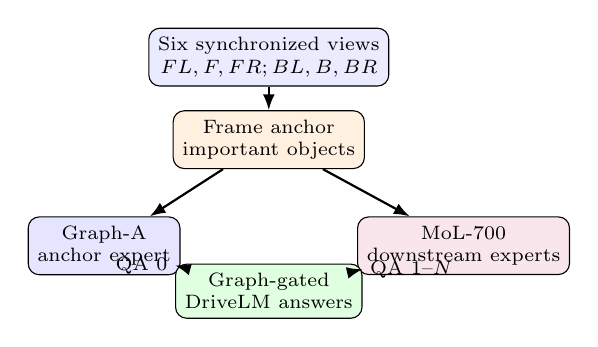
\begin{tikzpicture}[font=\scriptsize,node distance=3mm,
  box/.style={draw,rounded corners,align=center,minimum height=6mm},
  arr/.style={-{Latex[length=2mm]},thick}]
\node[box,fill=blue!8] (views) {Six synchronized views\\$FL,F,FR;BL,B,BR$};
\node[box,fill=orange!12,below=of views] (anchor) {Frame anchor\\important objects};
\node[box,fill=blue!10,below left=6mm and -1mm of anchor] (ga) {Graph-A\\anchor expert};
\node[box,fill=purple!10,below right=6mm and -1mm of anchor] (mo) {MoL-700\\downstream experts};
\node[box,fill=green!12,below=12mm of anchor] (out) {Graph-gated\\DriveLM answers};
\draw[arr] (views)--(anchor);
\draw[arr] (anchor)--(ga);
\draw[arr] (anchor)--(mo);
\draw[arr] (ga)--node[left]{QA 0}(out);
\draw[arr] (mo)--node[right]{QA 1--$N$}(out);
\end{tikzpicture}
\caption{Fixed node-level routing transferred from the complementary ensemble
observation in InternVL4Drive. Routing never reads a candidate answer or label.}
\label{fig:transfer}
\end{figure}

\subsection{Fixed node router}
For record $i$, the source is
\begin{equation}
s_i=\begin{cases}
\text{Graph-A}, & \texttt{qa\_index}_i=0,\\
\text{MoL-700}, & \text{otherwise}.
\end{cases}
\end{equation}
The rule routes exactly 467 frame anchors to Graph-A and 2,888 downstream QA
to MoL. It is independent of reference answers, candidate text, confidence,
and development score. Both source files have 3,355/3,355 coverage.

\subsection{Safety of semantic evaluation}
The local evaluator follows the public DriveLM structure,
\begin{equation}
F=.4J+.2L+.2M+.2A,
\end{equation}
where $J$ is semantic Planning score, $L$ combines BLEU-1--4, ROUGE-L and
CIDEr, $M$ combines coordinate F1 and graph semantics, and $A$ is exact
accuracy. DeepSeek-V4-Flash substitutes for the unavailable official GPT judge,
so we call the metric DriveLM-DS.

No new text is sent to an API. We implement a cache-only evaluator that does
not construct a network client, opens SQLite in read-only mode, reproduces the
frozen cache key, and fails on any miss. The promoted candidate obtains
791/791 cache hits and zero failures.

\section{Experiments}
\subsection{Setup}
The baseline is Qwen2.5-VL-7B with four task-specific rank-8 LoRA experts,
selected at MoL step 700. Graph-A is a shared Graph-SFT adapter trained for 600
updates over complete Perception--Prediction--Planning--Behavior frame
trajectories. Evaluation uses 3,355 scene-isolated QA. No model is retrained in
this experiment, making the attribution to routing exact.

We test two predeclared rules: (A) Graph-A only for the frame anchor; and (B)
Graph-A for the anchor and tag-3 grounding. Rule B has 132 semantic cache misses
and is therefore excluded rather than assigned an incomplete Final.

\subsection{Full-protocol result}
Table~\ref{tab:full} shows that the anchor ensemble increases eligible QA by 16,
improves Accuracy by 0.44 percentage points and semantic Planning by 0.54
points, and raises Final by 0.004048 (0.67\% relative). CIDEr slightly declines,
which is explicitly retained in the report.

\begin{table}[t]
\centering
\small
\caption{Complete 3,355-QA DriveLM-DS evaluation.}
\label{tab:full}
\begin{tabular}{lrrr}
\toprule
Metric & MoL-700 & v0.43 & $\Delta$\\
\midrule
Eligible & 1,911 & \textbf{1,927} & +16\\
Accuracy & 0.808735 & \textbf{0.813154} & +0.004419\\
Judge /100 & 72.4769 & \textbf{73.0197} & +0.5429\\
BLEU-1 & 0.772320 & \textbf{0.789634} & +0.017315\\
BLEU-2 & 0.709429 & \textbf{0.724770} & +0.015341\\
BLEU-3 & 0.651638 & \textbf{0.665099} & +0.013461\\
BLEU-4 & 0.595859 & \textbf{0.607520} & +0.011661\\
ROUGE-L & 0.723957 & \textbf{0.724571} & +0.000613\\
CIDEr & \textbf{0.200502} & 0.198875 & -0.001627\\
Match /100 & 30.7513 & 30.7513 & 0\\
Final & 0.608245 & \textbf{0.612293} & \textbf{+0.004048}\\
\bottomrule
\end{tabular}
\end{table}

\subsection{Same-ID audit}
Candidate-dependent graph gating can make raw Finals incomparable. We therefore
intersect the eligible IDs, yielding 1,848 common QA (633 tag-0, 616 tag-1, 467
tag-2, 132 tag-3). As Table~\ref{tab:paired} shows, every downstream metric is
identical because those answers are exactly MoL outputs. Only Language changes,
and Final still improves by 0.000993. All frozen promotion gates pass.

\begin{table}[t]
\centering
\small
\caption{Strict 1,848-ID paired audit.}
\label{tab:paired}
\begin{tabular}{lrrr}
\toprule
Metric & MoL-700 & v0.43 & $\Delta$\\
\midrule
Accuracy & 0.802528 & 0.802528 & 0\\
Planning /100 & 73.1169 & 73.1169 & 0\\
MC accuracy & 0.778966 & 0.778966 & 0\\
Coord. F1 & 0.146465 & 0.146465 & 0\\
Match /100 & 30.7513 & 30.7513 & 0\\
Language & 0.475440 & \textbf{0.480405} & +0.004965\\
Final & 0.609563 & \textbf{0.610557} & \textbf{+0.000993}\\
\bottomrule
\end{tabular}
\end{table}

The paired lexical Token-F1 decreases by 0.000969 and a separate token-level
ROUGE-L F1 decreases by 0.000474, although the official COCO Language aggregate
improves. This metric disagreement is a limitation, not omitted evidence.

\section{Discussion}
The result supports a specific interpretation of Graph-VQA: anchor perception
and downstream reasoning should not necessarily share one adapter. Graph-A
learns a better frame-level anchor representation, while MoL retains stronger
task-specialized reasoning. The fixed composition avoids the negative transfer
observed when Graph-SFT alone was used for every node.

This is not a parameter-level reproduction of InternVL4Drive and the scores are
not directly comparable. InternVL used 64 A100 GPUs, full-parameter tuning, an
official GPT judge and hidden leaderboard data. We use retained 7B LoRA models,
a local scene-isolated split and a DeepSeek proxy. What is reproduced is the
experimental principle of complementary specialization and ensembling.

\section{Next Steps}
We will evaluate three remaining transfers with equal-budget controls: (1)
explicit six-camera topology prompts while retaining six independent images;
(2) a labeled $2\times3$ mosaic plus global thumbnail with the same total visual
token budget; and (3) train-only point-to-box auxiliary grounding followed by
inverse conversion to official center coordinates. The promoted v0.43 output
should also be exported to official validation format and scored on the hidden
server before any leaderboard claim.

\section*{References}
\small
\begin{enumerate}
\item J. Li, Z. Li, and T. Lu. \emph{Driving with InternVL}. CVPR 2024
Autonomous Grand Challenge technical report, 2024.
\item C. Sima et al. \emph{DriveLM: Driving with Graph Visual Question
Answering}. ECCV, 2024.
\item Z. Chen et al. \emph{InternVL: Scaling up Vision Foundation Models and
Aligning for Generic Visual-Linguistic Tasks}. CVPR, 2024.
\item A. Kirillov et al. \emph{Segment Anything}. ICCV, 2023.
\end{enumerate}

\end{document}
